% Beyond the Lean Alone -- TMLR preprint style. Version en espanol. Compilar con latexmk -pdf
\documentclass[10pt]{article}
\usepackage[preprint]{tmlr}
\usepackage[utf8]{inputenc}
\usepackage[spanish,es-nodecimaldot,es-tabla]{babel}
\usepackage{etoolbox}
\makeatletter
\patchcmd{\abstract}{Abstract}{\abstractname}{}{}
\makeatother
\DeclareUnicodeCharacter{2212}{\ensuremath{-}}
\usepackage{amsmath,amssymb,mathtools}
\usepackage{booktabs,tabularx,array,graphicx}
\usepackage[shortlabels]{enumitem}
\usepackage{xcolor}
\definecolor{tinta}{HTML}{4F4086}
\usepackage[colorlinks=true,linkcolor=black,citecolor=tinta,urlcolor=tinta]{hyperref}
\usepackage{url}
\newcommand{\vr}[1]{\texttt{#1}}
\newcommand{\D}{\Delta}
\newcommand{\ic}[2]{[#1,\,#2]}
\newenvironment{idea}{\begin{quote}\noindent}{\end{quote}}
\newenvironment{pendiente}{\begin{quote}\small\noindent\textbf{Pendiente.}\ }{\end{quote}}

\title{Más allá del Lean solo: ¿separan linealmente los modelos de lenguaje congelados las formalizaciones adecuadas de las inadecuadas en Lean~4?}

\author{\name Carlos Manuel Orrego-Franco \email corregof@unal.edu.co \\
      \addr Departamento de Matem\'aticas y Estad\'istica\\
      Universidad Nacional de Colombia, Manizales
      \AND
      \name Juan Carlos Ria\~no-Rojas \email jcrianoro@unal.edu.co \\
      \addr Universidad Nacional de Colombia, Manizales
      \AND
      \name Fabi\'an Fernando Serrano-Su\'arez \email ffserranos@unal.edu.co \\
      \addr Universidad Nacional de Colombia, Manizales}

\begin{document}
\maketitle

\begin{abstract}
Una formalización en Lean puede compilar y, aun así, decir algo distinto del enunciado que debía capturar.
Preguntamos si las activaciones de modelos de lenguaje congelados separan linealmente las formalizaciones adecuadas
de las inadecuadas en Lean~4 \emph{más allá de lo que delata el Lean solo}. Medimos en tres niveles la brecha de
AUROC entre una sonda lineal que lee enunciado y formalización y otra que lee solo la formalización.
En 450 formalizaciones de CriticLeanBench, una réplica prerregistrada no pasó, porque ninguno de sus cuatro modelos
cumplió el criterio por modelo. Un bootstrap post hoc sitúa su brecha media en +0.045 (IC 95\% \ic{0.021}{0.069})
en una capa fija; en el último token el intervalo incluye el cero.
En 377 pares mínimos certificados por Lean, corridas exploratorias dieron una brecha positiva en tres de cuatro
modelos en el último token, pero frente al control de superficie más fuerte solo uno conserva un margen cuyo
intervalo excluye el cero.
En ProofNetVerif fue positiva en dos modelos, uno exploratorio.
Unos mapas exploratorios sitúan la separación sobre los tokens de Lean, en las capas superiores.
Las cifras son preliminares hasta compararlas con una implementación independiente escrita a mano.
Ningún nivel sostiene por sí solo la afirmación de que la adecuación es decodificable linealmente en modelos
congelados más allá del Lean solo. Lo leemos como una señal pequeña con factores de confusión conocidos, y
esbozamos una prueba confirmatoria con enunciados en Lean posteriores a los modelos y a este piloto.
\end{abstract}

\section{Introducción}

Un asistente de demostración comprueba que una demostración se sigue de un enunciado, pero que el enunciado sea el
que queríamos decir queda fuera de su alcance. Cuando un modelo de lenguaje traduce «toda sucesión monótona y acotada
converge» a Lean~4, el kernel aceptará cualquier proposición bien tipada, incluida una que omita la hipótesis de
acotación o cuantifique sobre el conjunto equivocado. A medida que la autoformalización crece en escala, los errores
de este tipo pueden esconderse allí donde un enunciado compila y no es el que se quería.

La mayor parte de los trabajos mide la adecuación (\emph{faithfulness}) desde afuera. Recurre a un modelo juez
\citep{criticlean,formalalign,zhang2026beyondcompilation,wang2026formalrx}, a una traducción de ida y vuelta al
lenguaje natural \citep{amrollahi2026roundtrip}, o a una comprobación de equivalencia con una formalización de
referencia \citep{proofnetverif,mohammad2026faithfulnessgap}. Nosotros miramos adentro. Preguntamos si un modelo
congelado, que nunca fue entrenado para juzgar formalizaciones, lleva ya una señal decodificable linealmente que
distingue una formalización adecuada de una inadecuada.

La dificultad está en que el texto en Lean es informativo por sí solo. Las formalizaciones inadecuadas difieren de
las adecuadas en estilo, longitud y vocabulario, y una sonda puede explotar esas diferencias sin relacionar en
absoluto el texto formal con el enunciado. Por esa razón nunca reportamos la AUROC de una sonda tomada aisladamente.
Cada resultado es una brecha, es decir, la AUROC de una sonda que lee el enunciado junto con el Lean menos la de
una sonda que lee solo el Lean. Una brecha positiva es evidencia de que la representación lleva información sobre la
\emph{relación} entre los dos textos.

Decimos «separa» y «es decodificable linealmente» en todo el texto, porque una sonda lineal es correlacional. Que
una dirección separe dos clases no muestra que el modelo la use.

\paragraph{Contribuciones.}
\begin{enumerate}
\item Un diseño en tres niveles en el que cada nivel elimina un factor de confusión del anterior. El Nivel~A tiene
etiquetas validadas por humanos en un benchmark público. El Nivel~B tiene pares mínimos con no equivalencia
certificada por Lean y el mismo enunciado en ambos miembros. El Nivel~C tiene un benchmark etiquetado de forma
independiente, con una prueba de transferencia.
\item Un control de \emph{superficie cruzada}, construido con rasgos que cruzan el enunciado y el texto formal. En el
modelo donde separamos por tipo de edición, iguala a las activaciones en los cambios de numeral, que una línea de
base de superficie limitada al Lean habría pasado por alto. En conjunto, sin embargo, los n-gramas simples de ambos
textos son el control más fuerte en nuestros pares.
\item Una réplica prerregistrada. Ningún modelo cumplió su criterio por modelo, aunque la brecha media de los cuatro
modelos es positiva con la lectura de capa fija.
\item La datación de cada origen del Nivel~B frente al lanzamiento de cada modelo, y un borrador de protocolo
confirmatorio restringido a enunciados escritos después (Apéndice~\ref{app:protocolo}).
\item Mapas exploratorios por capa y posición de la dirección de la sonda en cinco modelos, un análisis en el
espíritu del mapeo basado en información \citep{searchlight}. Muestran dónde la etiqueta es legible linealmente con
el enunciado y sin él.
\end{enumerate}

% ------------------------------------------------------------------ 2
\section{Trabajos relacionados}

\paragraph{El antecedente más cercano.}
El trabajo más cercano al nuestro es el de \citet{genv}, que entrenan un verificador generativo para la
autoformalización a SMT-LIB, destilado de un oráculo de equivalencia de Z3. Le dan nombre a la falla que
estudiamos, traducciones que se ejecutan y coinciden con el veredicto esperado pero siguen siendo incorrectas, y
además leen su verificador desde adentro. Una sonda lineal sobre los códigos de autoencoder disperso de su flujo
residual alcanza 0.960 de AUROC, y las sondas sobre los estados ocultos de sus líneas de base con ajuste fino
separan mejor que las salidas de esas mismas líneas de base. Sus modelos, sin embargo, están entrenados para
juzgar, y su escenario son problemas de lógica en SMT-LIB. Los nuestros son modelos congelados que nunca fueron
entrenados para la tarea, y el lenguaje formal es Lean~4. Medimos, además, cada resultado contra lo que el texto
formal separa por sí solo en el nivel de las representaciones.

\paragraph{La adecuación medida desde afuera.}
Los trabajos que miden la adecuación desde afuera nos dan también dos de nuestros benchmarks.
FormalAlign \citep{formalalign} puntúa la alineación entre un enunciado y su formalización con un modelo entrenado
para ese fin. CriticLean \citep{criticlean} entrena un crítico para juzgar formalizaciones en Lean~4 e introduce
CriticLeanBench, que usamos en el Nivel~A. \citet{proofnetverif} estudian métricas de evaluación para la
autoformalización de enunciados y publican ProofNetVerif, que usamos en el Nivel~C.

\paragraph{Estados ocultos y corrección.}
Decodificar la corrección a partir de los estados ocultos tiene antecedentes. Las propiedades afines a la verdad
son decodificables linealmente en lenguaje natural \citep{geometry}, aunque esas sondas no tienen por qué
generalizar de un conjunto de datos a otro \citep{orgad}. La corrección del código también se ha decodificado de
los estados ocultos antes de la generación \citep{dicicco}. Por eso no reclamamos como nuestra la observación de
que el interior de un modelo puede separar más de lo que su salida expresa. Nuestra línea de base de solo Lean
cumple el papel que en esa literatura cumplen los controles de longitud y de superficie.

\paragraph{Decodificable no significa usado.}
\citet{decodability} sondean la validez lógica en cinco modelos de pesos abiertos y luego ponen a prueba si
intervenir sobre la información decodificada cambia el comportamiento. Leemos nuestros propios resultados bajo la
advertencia de su título y no hacemos ninguna afirmación causal.

\paragraph{Una nota sobre los términos.}
En inglés, \emph{faithfulness} nombra también la fidelidad de las explicaciones de \emph{chain-of-thought}. Aquí
«adecuación» significa únicamente que una formalización dice lo que dice el enunciado en lenguaje natural.

% ------------------------------------------------------------------ 3
\section{Método}

\paragraph{Sonda.}
Para cada modelo, capa y variante del prompt leemos las activaciones del flujo residual del modelo congelado y
ajustamos una regresión logística estandarizada ($C = 1$). Todos los puntajes son \emph{out-of-fold}, con las
particiones agrupadas de modo que ningún enunciado aparezca a ambos lados de una división. No se actualiza ningún
peso del modelo.

\paragraph{Variantes del prompt.}
La sonda lee uno de cuatro prompts. \vr{full} contiene el enunciado, la formalización en Lean y la pregunta
«Is this formalization faithful?». \vr{lean\_only} es el mismo prompt sin el enunciado, y \vr{nl\_only} es el mismo
sin el Lean. \vr{nl\_mismatched} empareja el Lean con el enunciado de otro problema de longitud similar.

\paragraph{Lecturas.}
Leemos las activaciones de dos maneras. La lectura~(i) toma el último token del prompt, con la capa elegida por
validación cruzada anidada. La lectura~(ii) toma la media sobre los tokens de Lean en una capa fijada de antemano,
$\lfloor 2L/3 \rfloor$.

\paragraph{Estadístico central.}
El estadístico central es la brecha
$\D = \mathrm{AUROC}(\vr{full}) - \mathrm{AUROC}(\vr{lean\_only})$, que reportamos con un intervalo bootstrap del 95\% sobre grupos \citep{efron}.
En el Nivel~B la AUROC es \emph{pareada}. Es la probabilidad de que el miembro adecuado de un par puntúe por encima
de su gemelo inadecuado, promediada dentro de cada origen y luego sobre los orígenes. El remuestreo sigue allí la
misma estructura, de modo que el bootstrap remuestrea orígenes, las particiones se agrupan por archivo fuente y la
prueba de permutación intercambia los papeles dentro de cada par.

\begin{table}[h]
\centering
\caption{Controles. Donde un control se corrió, se reporta como \vr{full} menos el control; no todos se corrieron en todos los niveles.}
\label{tab:controles}
\vspace{2pt}
\begin{tabularx}{\linewidth}{@{}lX@{}}
\toprule
Control & Qué descarta\\
\midrule
Superficie: n-gramas del Lean y del enunciado & separación por vocabulario, longitud o estilo de cualquiera de los dos textos\\
Superficie cruzada: rasgos que cruzan los dos textos & un token presente en el Lean y ausente del enunciado (un numeral, una relación)\\
Apilado: sondas \vr{lean\_only} + \vr{nl\_only} & separación que no requiere interacción entre los dos textos\\
\vr{nl\_mismatched} & una ganancia debida a la presencia de \emph{cualquier} enunciado, y no del correcto\\
P(Yes) & que la propia respuesta de sí o no del modelo ya lleve la señal\\
Pesos aleatorios & separación producida solo por la arquitectura y el tokenizador\\
Embeddings de oraciones (bge-m3) & separación al alcance de un codificador genérico\\
\bottomrule
\end{tabularx}
\end{table}

\paragraph{Estimación.}
Usamos cinco particiones, estratificadas por etiqueta y agrupadas por enunciado normalizado, y repetimos todo el
procedimiento con cinco semillas. La puntuación de una fila es la media de sus puntuaciones \emph{out-of-fold}
sobre las semillas. Los intervalos salen de 2000 remuestreos bootstrap de grupos, estratificados por clase. La
prueba de permutación del Nivel~A baraja las etiquetas 1000 veces con las particiones fijas y repite cada vez el
procedimiento entero, incluida la selección de capa. Es unilateral, con
$p = (1 + \#\{\D_{\mathrm{perm}} \ge \D_{\mathrm{obs}}\})/1001$. En todo el texto, $L$ es el número de bloques del
transformer, de modo que la capa fija es la 21 de 32 en OLMo-2.

\paragraph{Modelos.}
Sondeamos cinco modelos de propósito general: Qwen3-4B y Qwen3-8B \citep{qwen3}, OLMo-2-7B \citep{olmo2},
Gemma-3-4B \citep{gemma3} y Llama-3.1-8B \citep{llama3}. A ellos se suman tres modelos entrenados para Lean:
DeepSeek-Prover-V2-7B \citep{deepseekproverv2}, Goedel-Prover-V2-8B \citep{goedelproverv2} y
Kimina-Autoformalizer-7B \citep{kimina,kiminaautoformalizer}. Todos corren localmente en bfloat16, con
revisiones fijadas (Apéndice~\ref{app:modelos}).

\paragraph{Lo que se fijó de antemano.}
Cada nivel tiene una regla de decisión escrita, con su SHA-256 y su hora de aprobación registrados. Estas reglas son
archivos internos, con hash y sello de tiempo, guardados en la bitácora del proyecto. No son entradas de un registro
público, y «prerregistrado» se usa en ese sentido en todo el texto. El Nivel~A se prerregistró antes de correr
cualquiera de sus cuatro modelos de réplica. Las reglas de los Niveles~B y~C se aprobaron antes de sus análisis, y
el Nivel~B se declara exploratorio. Las decisiones tomadas después de ver un resultado se listan en el
Apéndice~\ref{app:desviaciones}.

\begin{pendiente}
Todas las cifras de este borrador provienen de la implementación de referencia y son preliminares. Por la regla del
proyecto, solo pasan a ser hallazgos tras compararlas con la implementación a mano del propio primer autor
(\vr{probe.py}), que aún no está escrita. El Nivel~C tiene además una segunda implementación, escrita por otro agente
de programación, sin acceso a la primera y a partir de las mismas activaciones extraídas. Reproduce el resultado
principal de ese nivel.
\end{pendiente}

% ------------------------------------------------------------------ 4
\section{Nivel A: CriticLeanBench y una réplica prerregistrada}

\begin{figure}[t]
\centering
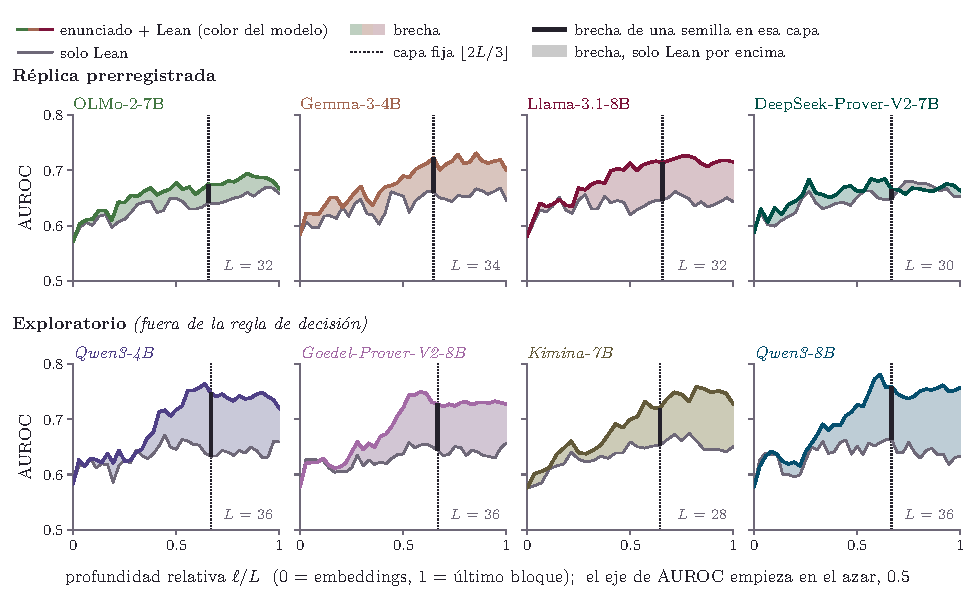
\includegraphics[width=\linewidth]{figuras_v3/curvas_por_modelo_es.pdf}
\caption{Capa por capa. AUROC de una sonda lineal que lee el enunciado con el Lean (cada modelo en su propio color) y el Lean solo (gris) en las 450 formalizaciones de CriticLeanBench, media sobre los tokens de Lean; el área sombreada es su brecha, gris donde el Lean solo queda por encima. La línea punteada marca la capa fijada de antemano para la lectura~(ii), $\lfloor 2L/3 \rfloor$, y el segmento negro es una versión, con una sola semilla, de la brecha que esa lectura mide. Fila superior: la réplica prerregistrada. Fila inferior: modelos exploratorios. Descriptiva: una semilla, sin selección de capa, sin intervalos; nada en el artículo se decide a partir de esta figura.}
\label{fig:relieve}
\end{figure}


\paragraph{Datos.}
El Nivel~A usa las 450 formalizaciones de CriticLeanBench que compilan \citep{criticlean}, de las cuales 250 son
adecuadas y 200 inadecuadas. Sus etiquetas fueron propuestas por un modelo y validadas por revisores humanos.

\paragraph{Descubrimiento.}
El efecto se vio primero en un solo modelo. La primera corrida fue en Qwen3-4B, en el último token, con selección
anidada de capa y 100 permutaciones. Dio
$\D$ = +0.088 \ic{0.039}{0.134} con $p = 0.0099$ de permutación, el menor valor que 100 permutaciones pueden devolver. Dos
modelos entrenados para Lean, Goedel-Prover-V2 y Kimina, se corrieron después bajo la misma regla temprana. Sus intervalos
bootstrap excluían el cero, pero los valores $p$ de permutación de la diferencia fueron 0.16 y 0.25. Ese desacuerdo
llevó a la regla más estricta que sigue, la tercera versión escrita ese día. Estas corridas no tienen peso
confirmatorio.

Recalculados con el pipeline prerregistrado, los tres modelos de descubrimiento dan +0.091, +0.043 y +0.044 con la
lectura~(i), y +0.095, +0.066 y +0.051 con la lectura~(ii). El enunciado solo ya predice la etiqueta, pues
\vr{nl\_only} alcanza de 0.61 a 0.74 en los cuatro modelos de réplica. Por esa razón cada brecha se compara también
con un control apilado.

\paragraph{Prerregistro.}
El prerregistro se firmó el 4 de noviembre de 2026 a las 22:29 (UTC$-$5), antes de correr cualquiera de los cuatro
modelos nuevos. Según su regla, un modelo pasa si se cumplen dos condiciones en cualquiera de las dos lecturas. La
condición~(a) es que su valor $p$ con 1000 permutaciones quede por debajo de 0.05 tras la corrección de Holm
\citep{holm} sobre las ocho pruebas (cuatro modelos, dos lecturas). Cada permutación baraja las etiquetas, reajusta
las dos sondas y recalcula $\D$. La condición~(b) es que el intervalo de \vr{full} menos apilado quede por completo
por encima de cero. La afirmación global se sostiene si al menos tres de los cuatro modelos pasan y el intervalo de
efectos aleatorios queda por encima de cero en la misma lectura.

Dos cláusulas de esta regla las confirmó el primer autor el 5 de noviembre, cuando ya se habían visto los
resultados de la lectura~(ii). Una es que un modelo pueda pasar con cualquiera de las lecturas, y la otra, que la
afirmación global se lea dentro de una sola lectura. Ninguna cambia un umbral numérico, aunque la primera decide si
un modelo debe pasar en una lectura o en las dos, y las registramos como una desviación.

La prueba de permutación y el intervalo bootstrap responden preguntas distintas. La primera reajusta las sondas con
las etiquetas barajadas, mientras que el segundo remuestrea grupos con las puntuaciones ya ajustadas. Por eso la
Tabla~\ref{tab:a} puede mostrar un intervalo que excluye el cero junto a $p = 0.040$.

\begin{table}[h]
\centering
\caption{Nivel A, modelos prerregistrados. Con ocho pruebas, el menor $p$ crudo debe caer por debajo de 0.00625 para
sobrevivir a Holm; el menor observado es 0.040 (0.32 tras el ajuste). Dos pruebas de permutación de la lectura~(i) no se corrieron porque la condición~(b)
ya fallaba allí y no podían cambiar la decisión.}
\label{tab:a}
\vspace{2pt}
{\small\setlength{\tabcolsep}{4pt}
\begin{tabular}{@{}lccccc@{}}
\toprule
 & \vr{full} & \vr{lean\_only} & $\D$ [IC 95\%] & \vr{full} $-$ apilado [IC 95\%] & $p$ (crudo)\\
\midrule
\multicolumn{6}{@{}l}{\emph{Lectura (ii): media sobre los tokens de Lean, capa fija}}\\
OLMo-2-7B             & 0.724 & 0.679 & +0.044 [+0.009, +0.079] & +0.049 [+0.014, +0.083] & 0.084\\
Gemma-3-4B            & 0.745 & 0.688 & +0.058 [+0.021, +0.094] & +0.067 [+0.030, +0.102] & 0.040\\
Llama-3.1-8B          & 0.736 & 0.682 & +0.054 [+0.018, +0.088] & +0.056 [+0.021, +0.089] & 0.040\\
DeepSeek-Prover-V2-7B & 0.704 & 0.678 & +0.025 [−0.008, +0.061] & +0.033 [−0.001, +0.067] & 0.191\\
\midrule
\multicolumn{6}{@{}l}{\emph{Lectura (i): último token, capa por validación cruzada anidada}}\\
OLMo-2-7B             & 0.738 & 0.705 & +0.032 [−0.011, +0.075] & +0.032 [−0.007, +0.069] & 0.195\\
Gemma-3-4B            & 0.726 & 0.688 & +0.038 [−0.009, +0.085] & +0.013 [−0.029, +0.055] & no corrida\\
Llama-3.1-8B          & 0.712 & 0.723 & −0.011 [−0.056, +0.031] & −0.059 [−0.098, −0.021] & no corrida\\
DeepSeek-Prover-V2-7B & 0.684 & 0.627 & +0.056 [+0.008, +0.104] & +0.043 [+0.003, +0.085] & 0.084\\
\bottomrule
\end{tabular}}
\end{table}

\paragraph{Decisión.}
Ningún modelo pasa. Con la lectura~(ii) el intervalo de \vr{full} menos apilado excluye el cero en tres de los cuatro
modelos, de modo que la condición~(b) se cumple en gran medida. Ningún modelo, sin embargo, sobrevive a la prueba de
permutación corregida por multiplicidad. Con la lectura~(i) solo DeepSeek-Prover-V2 cumple la condición~(b), con
$p = 0.084$. El análisis de sensibilidad previsto retira las 44 filas cuyas etiquetas habíamos marcado como
dudosas, con lo que quedan 406 filas. Deja igual la lectura~(ii), con brechas de +0.046, +0.060, +0.060 y +0.030
\ic{−0.006}{0.065}, en el orden de la Tabla~\ref{tab:a}.

\paragraph{Metaanálisis.}
La estimación prerregistrada de DerSimonian--Laird \citep{dl} sobre los cuatro modelos nuevos es +0.045 \ic{0.027}{0.062} con
la lectura~(ii), con $\tau^2 = 0$ e $I^2 = 0\%$. Con la lectura~(i) es +0.028 \ic{−0.000}{0.056} ($I^2 = 34\%$).
Al añadir los tres modelos de descubrimiento se obtiene +0.056 \ic{0.041}{0.071} con~(ii) ($I^2 = 25\%$), pero esa
cifra es exploratoria, porque incluye el modelo en el que se halló el efecto.

El intervalo de efectos aleatorios es demasiado estrecho, porque los cuatro modelos se puntuaron sobre las mismas
450 formalizaciones y sus estimaciones no son independientes. Un bootstrap post hoc atiende ese problema al
remuestrear los mismos grupos conjuntamente para los cuatro modelos, con 2000 remuestreos estratificados por
clase. Sitúa su brecha media en +0.045 \ic{0.021}{0.069} con~(ii) y en +0.029 \ic{−0.000}{0.058} con~(i). Lo que
estima es la brecha media de estos cuatro modelos sobre la población de ítems, con los modelos fijos, así que no
dice nada sobre un quinto modelo.

\begin{figure}[t]
\centering
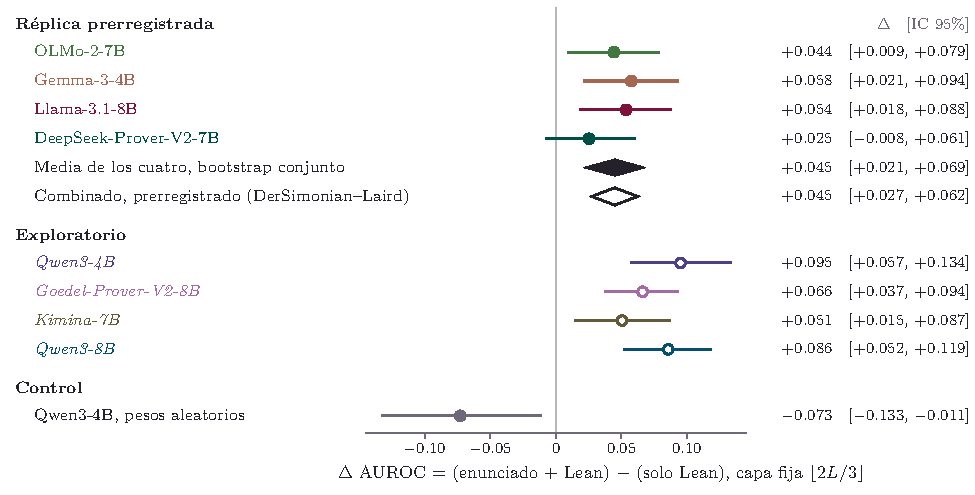
\includegraphics[width=\linewidth]{figuras_v3/forest_nivel_a_es.pdf}
\caption{Nivel A, lectura (ii). Puntos llenos: los cuatro modelos prerregistrados. Rombo lleno: su media, con el bootstrap conjunto post hoc sobre ítems; rombo vacío: la estimación prerregistrada de DerSimonian--Laird. Puntos vacíos: modelos exploratorios. Gris: la misma arquitectura con pesos aleatorios. Cada modelo conserva su color en todas las figuras.}
\label{fig:forest}
\end{figure}

\paragraph{Controles nulos.}
Dos controles nulos comprueban si la arquitectura por sí sola, o un codificador genérico, producirían la brecha.
Con pesos aleatorios, Qwen3-4B da +0.008 \ic{−0.041}{0.056} con~(i) y −0.073 \ic{−0.133}{−0.011} con~(ii).
Sobre los embeddings de oraciones de bge-m3 \citep{bgem3} la brecha es −0.098 \ic{−0.153}{−0.044}. Ninguno de los
dos la produce.

\paragraph{Un modelo exploratorio posterior.}
Qwen3-8B se añadió después y es exploratorio. Da +0.043 \ic{−0.004}{0.088} con~(i) y +0.086 \ic{0.052}{0.119}
con~(ii), con \vr{full} menos apilado en +0.113 \ic{0.078}{0.148} con~(ii). No se corrieron permutaciones.

\paragraph{La fuente del problema.}
CriticLeanBench toma sus problemas de doce fuentes, y la proporción de formalizaciones adecuadas difiere de una a
otra. En consecuencia, la fuente sola separa las etiquetas con AUROC 0.578 \ic{0.525}{0.629}. Un análisis post hoc,
hecho solo con la lectura~(ii), pregunta si la brecha es la fuente leída por otra vía. Una fuente, AIME, no tiene
ítems adecuados (0 de 3) y no aporta nada.

La primera comprobación compara las formalizaciones adecuadas e inadecuadas solo dentro de la misma fuente y
combina la comparación sobre las fuentes. La brecha media de los cuatro modelos prerregistrados con la
lectura~(ii) es entonces +0.049 \ic{0.021}{0.079}. Modelo por modelo, esta brecha dentro de la fuente es +0.052
\ic{0.006}{0.097} en OLMo-2, +0.081 \ic{0.035}{0.127} en Gemma-3, +0.052 \ic{0.009}{0.096} en Llama-3.1 y +0.013
\ic{−0.027}{0.053} en DeepSeek-Prover-V2.

La segunda comprobación entrena la sonda con once fuentes y la prueba en la duodécima. Da una brecha de +0.079
\ic{0.031}{0.130} en OLMo-2, +0.091 \ic{0.039}{0.141} en Gemma-3, +0.104 \ic{0.054}{0.155} en Llama-3.1 y +0.043
\ic{−0.002}{0.088} en DeepSeek-Prover-V2. Las puntuaciones de la fuente apartada se comparan solo dentro de esa
fuente, en la capa fija y con un ajuste por fuente. Estas brechas son mayores que las de la Tabla~\ref{tab:a}
porque \vr{lean\_only} pierde más que \vr{full} cuando la fuente se aparta. En Llama-3.1, por ejemplo,
\vr{lean\_only} cae de 0.659 dentro de la fuente a 0.596, mientras que \vr{full} pasa de 0.710 a 0.700. La sonda
que lee solo el Lean se apoya en rasgos propios de cada fuente.

\paragraph{Dónde es legible la separación.}
La Figura~\ref{fig:escaner} aplica la dirección de la sonda de cada capa, ajustada sin la fila en cuestión, a los
tokens de cada posición del prompt. El análisis sigue el espíritu del mapeo basado en información (\emph{searchlight})
\citep{searchlight}, con una diferencia. En lugar de ajustar un clasificador en cada posición, aplicamos una única
dirección, ajustada sobre la media de los tokens de Lean, posición por posición. Los mapas sobre capas y posiciones
de token son un recurso habitual en interpretabilidad, construidos por lo general a partir de intervenciones
causales \citep{meng2022rome,geometry} o de direcciones de lectura \citep{zou2023repe}. El nuestro muestra dónde la
etiqueta es legible linealmente. No muestra dónde se calcula la etiqueta ni si el modelo la usa. Como relee los
datos de la lectura~(ii), tampoco es una prueba independiente.

En los cinco modelos de propósito general esta dirección, ajustada sobre los tokens de Lean, está en el azar o cerca
de él sobre el tramo del enunciado, donde el modelo aún no ha leído el Lean. En promedio queda allí entre 0.49 y
0.52, y la única excepción es Qwen3-8B, con 0.521 \ic{0.501}{0.543}. Después sube sobre los tokens de Lean en las
capas superiores. Eso no significa que el enunciado no lleve información sobre la etiqueta, pues las sondas
\vr{nl\_only} alcanzan de 0.61 a 0.74.

Sobre los tokens de Lean, la separación es más débil en cuatro de los cinco modelos cuando se retira el enunciado.
Promediada sobre esos tokens en el 60\% superior de las capas, la AUROC por celda con el enunciado supera a la que
se obtiene sin él en +0.043 \ic{0.032}{0.054} en Qwen3-8B, +0.039 \ic{0.028}{0.050} en Qwen3-4B, +0.031
\ic{0.019}{0.043} en Llama-3.1, +0.024 \ic{0.014}{0.035} en Gemma-3 y +0.012 \ic{−0.001}{0.024} en OLMo-2. Los
intervalos salen de 300 remuestreos de filas con las direcciones fijas. Bajo un nulo pareado que intercambia las
dos condiciones dentro de cada fila, con 500 intercambios, el percentil 95 de esa diferencia es a lo sumo 0.011.
Ese nulo da $p = 0.002$ en cuatro modelos, el menor valor que pueden devolver 500 intercambios, y $p = 0.022$ en
OLMo-2. En OLMo-2 los dos procedimientos discrepan, pues su intervalo incluye el cero, y en ese modelo tratamos la
diferencia como no establecida. La región, además, se eligió después de ver los mapas, y la dirección se ajustó
sobre la media de los tokens de Lean y se aplicó token por token. Los mapas son exploratorios.

\paragraph{Interpretación.}
El efecto tal como se prerregistró, modelo por modelo, no se confirmó. Con 450 filas por modelo, el instrumento no
resuelve una brecha de este tamaño después de la corrección. El bootstrap conjunto post hoc sitúa la brecha media
de los cuatro modelos nuevos en +0.045 \ic{0.021}{0.069} con la lectura de capa fija y en +0.029
\ic{−0.000}{0.058} con la lectura en el último token, y ninguno de los dos controles nulos muestra una brecha
positiva. Esto no es una réplica bajo la regla que escribimos.
La Figura~\ref{fig:relieve} muestra los mismos datos capa por capa.

\begin{figure}[t]
\centering
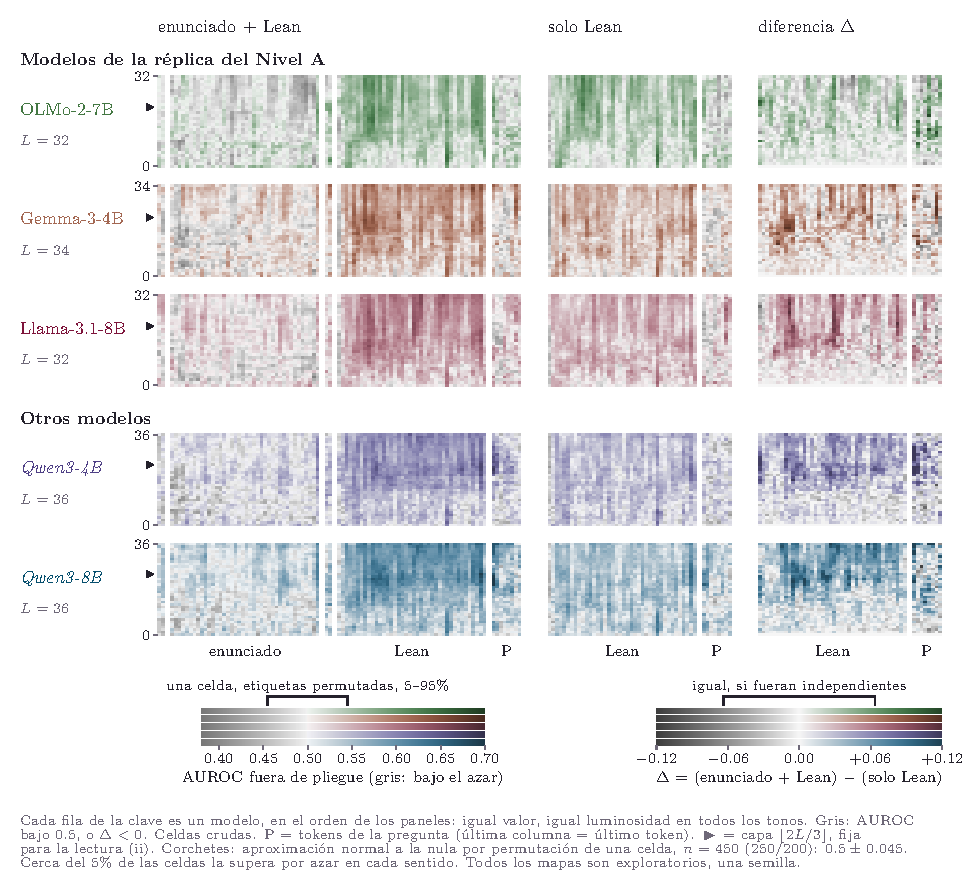
\includegraphics[width=\linewidth]{figuras_v3/escaner2d_modelos_es.pdf}
\caption{En qué parte del prompt y a qué profundidad es legible la separación, en los cinco modelos de propósito general. Cada celda es la AUROC \emph{out-of-fold} de la dirección de la sonda de la capa, aplicada a los tokens de esa posición, en las 450 formalizaciones de CriticLeanBench; los tramos se estiran a un ancho fijo y las celdas van crudas. Izquierda: el prompt con enunciado y Lean. Centro: el Lean solo. Derecha: su diferencia, en el color del modelo donde el enunciado suma y en gris donde resta. Todos los modelos comparten una misma escala de luminosidad, de modo que valores iguales son igual de oscuros; las celdas por debajo del azar son grises. Los corchetes sobre las claves dan el tamaño del ruido de una sola celda por una aproximación normal y, para la diferencia, una cota de independencia. El marcador es la capa $\lfloor 2L/3 \rfloor$. Exploratoria: una semilla, una dirección ajustada sobre la media de los tokens de Lean y aplicada token por token.}
\label{fig:escaner}
\end{figure}

% ------------------------------------------------------------------ 5
\section{Nivel B: pares mínimos certificados por Lean}

\paragraph{Construcción.}
Cada par reúne dos ediciones mínimas del mismo enunciado original en Lean. Lean certifica una de ellas como
equivalente al original, y esa edición es el miembro adecuado. Certifica la otra como no equivalente, y esa es el
miembro inadecuado. El enunciado en lenguaje natural es idéntico en ambos, así que el enunciado solo no puede
separarlos. La sonda \vr{nl\_only} da, en consecuencia, 0.500 por construcción, lo que sirve de comprobación del
pipeline.

Las ediciones inadecuadas caen en tres familias. La familia A hace el teorema más fuerte, B lo hace más débil y C
lo convierte en un teorema distinto. Dentro de C, C2 cambia un numeral y C3 cambia otra cosa.

Los orígenes provienen de formal-conjectures \citep{fc,fcpaper} (323 pares) y de
FormalMATH-Lite \citep{formalmath} (54 pares). Tras las exclusiones fijadas antes de extraer cualquier activación, el
lote principal tiene 377 pares de 256 orígenes en 189 archivos fuente, certificados con Lean~4.34.1 \citep{lean4,mathlib}.
Lean certificó 408 pares. Una revisión hecha por un modelo de lenguaje, no por una persona, encontró después
originales que no eran adecuados a su enunciado y ediciones que eran equivalentes de hecho, y esos 31 pares se
retiraron. Como referencia, con los 408 la brecha en Qwen3-4B es +0.213 \ic{0.150}{0.280}.

El lote queda por debajo de los 400 pares y los 300 orígenes que pedía la regla, y eso es lo que significa
«potencia reducida» en la Tabla~\ref{tab:b}. Por la misma regla, un modelo cuyo intervalo de $\D$ incluye el cero
se registra como nulo con su cota superior. La regla, además, solo permite escribir «más allá de la superficie»
cuando el intervalo de \vr{full} menos superficie cruzada queda por encima de cero. La prueba prevista al principio
para este nivel usaba tripletas. No se pudo construir un lote certificable de tripletas, y los pares se declararon
lote de desarrollo.

\begin{table}[h]
\centering
\caption{Nivel B, 377 pares. Arriba: la prueba central, AUROC pareada en el último token. Con 100 permutaciones dentro de cada par, el
menor $p$ alcanzable es 0.0099; la prueba de permutación usa el estadístico de la semilla 0 (0.250, 0.118, 0.104 y 0.079), mientras que la columna $\D$ es la estimación con cinco semillas. Por la regla, las tres primeras filas son positivas con potencia reducida y la cuarta es
un nulo con cota superior 0.107.}
\label{tab:b}
\vspace{2pt}
\begin{tabular}{@{}lcccc@{}}
\toprule
 & \vr{full} & \vr{lean\_only} & $\D$ [IC 95\%] & $p$ ($\D$)\\
\midrule
Qwen3-4B     & 0.807 & 0.582 & +0.225 [+0.158, +0.291] & 0.0099\\
OLMo-2-7B    & 0.766 & 0.664 & +0.102 [+0.039, +0.164] & 0.0198\\
Llama-3.1-8B & 0.762 & 0.678 & +0.084 [+0.023, +0.146] & 0.0198\\
Gemma-3-4B   & 0.684 & 0.643 & +0.041 [−0.023, +0.107] & 0.0594\\
\midrule
\multicolumn{5}{@{}l}{\emph{Segunda lectura: media sobre los tokens de Lean (sin prueba de permutación)}}\\
Qwen3-4B     & 0.944 & 0.780 & +0.164 [+0.120, +0.210] & ---\\
OLMo-2-7B    & 0.859 & 0.775 & +0.084 [+0.039, +0.129] & ---\\
Llama-3.1-8B & 0.902 & 0.768 & +0.135 [+0.090, +0.180] & ---\\
Gemma-3-4B   & 0.895 & 0.777 & +0.117 [+0.072, +0.162] & ---\\
\bottomrule
\end{tabular}
\end{table}

\begin{table}[h]
\centering
\caption{Controles del Nivel B, todos en el último token. Los clasificadores de n-gramas y de superficie cruzada alcanzan por sí solos 0.729 y 0.688. La última columna repite la prueba central en los 309 pares que quedan al retirar las
ediciones de numeral (C2).}
\label{tab:bcontroles}
\vspace{2pt}
{\footnotesize\setlength{\tabcolsep}{3pt}
\begin{tabular}{@{}lcccc@{}}
\toprule
\vr{full} menos & n-gramas & superficie cruzada & P(Yes) & sin C2, frente a \vr{lean\_only}\\
\midrule
Qwen3-4B     & +0.078 [+0.010, +0.141] & +0.118 [+0.058, +0.177] & −0.032 [−0.074, +0.008] & +0.187 [+0.112, +0.260]\\
OLMo-2-7B    & +0.037 [−0.023, +0.094] & +0.077 [+0.018, +0.135] & +0.040 [−0.010, +0.091] & +0.073 [+0.006, +0.139]\\
Llama-3.1-8B & +0.033 [−0.035, +0.098] & +0.073 [+0.012, +0.133] & +0.033 [−0.022, +0.085] & +0.019 [−0.049, +0.088]\\
Gemma-3-4B   & −0.045 [−0.107, +0.018] & −0.005 [−0.066, +0.060] & +0.124 [+0.062, +0.189] & +0.002 [−0.071, +0.077]\\
\bottomrule
\end{tabular}}
\end{table}

\paragraph{Lo que dicen los controles.}
El primer control cambia el enunciado por uno equivocado. Con él la sonda cae al azar en todos los modelos (0.506 a
0.537), de modo que la ganancia requiere el enunciado \emph{correcto}. Frente al control de superficie cruzada, tres
modelos conservan un margen positivo y Gemma no. En este lote, sin embargo, los n-gramas simples de los dos textos
separan los pares mejor (0.729) que los rasgos de superficie cruzada (0.688), así que son el control más exigente
en conjunto. Frente a ellos solo Qwen3-4B conserva un margen (+0.078 \ic{0.010}{0.141}), y en los otros tres el
intervalo incluye el cero. En las ediciones de numeral que se examinan más abajo, en cambio, los rasgos de
superficie cruzada alcanzan 0.933, cosa que los n-gramas no logran.

La propia respuesta del modelo pone otro límite. En Qwen3-4B su respuesta de sí o no separa los pares tan bien como
la sonda (0.839 frente a 0.807), de modo que allí la sonda no añade nada detectable sobre esa respuesta. En el
último token, ningún modelo supera a la vez el control de n-gramas y su propio P(Yes) con intervalos por encima de
cero. Un control adicional, también en Qwen3-4B, puntúa el original sin editar frente a su edición adecuada y los
encuentra indistinguibles (0.520), lo que descarta que la señal sea «haber sido editado».

\paragraph{La segunda lectura.}
Todos los controles del Nivel~B se calcularon solo frente a la sonda del último token, y ninguno se calculó para la
segunda lectura. La brecha sobre el Lean solo sí se midió en ambas, y depende también de la lectura. En la media
sobre los tokens de Lean es positiva en los cuatro modelos, con +0.164 \ic{0.120}{0.210} en Qwen3-4B, +0.084
\ic{0.039}{0.129} en OLMo-2, +0.135 \ic{0.090}{0.180} en Llama-3.1 y +0.117 \ic{0.072}{0.162} en Gemma-3. El nulo
de Gemma-3 es, por tanto, específico del último token.

Con esa lectura, sin embargo, el propio \vr{lean\_only} es mucho más alto (0.77 a 0.78), así que el Lean solo
delata más de lo que sugiere la Tabla~\ref{tab:b}. Una sonda que lee solo el Lean y llega a 0.78 en pares que
comparten un mismo enunciado queda por encima de la línea base de n-gramas de ambos textos (0.729). Los n-gramas,
por tanto, no recogen todo lo que el texto en Lean revela sobre cuál de las dos ediciones es la inadecuada. Con
esta lectura no se corrió ninguna prueba de permutación.

\paragraph{El efecto se concentra en la familia C, y en Qwen3-4B las ediciones de numeral dentro de C son un efecto de superficie.}
Frente al Lean solo, la familia C da la brecha más grande en los cuatro modelos (Tabla~\ref{tab:bfam}). En las
familias A y B el intervalo excluye el cero solo en Qwen3-4B y, para la familia A, en OLMo-2, mientras que
Llama-3.1 y Gemma-3 quedan a menos de 0.023 del cero.
Una división post hoc en Qwen3-4B (Figura~\ref{fig:b}, abajo) muestra por qué. En C2 el control de superficie cruzada
alcanza 0.933 por sí solo, lo que es indistinguible de las activaciones, que dan 0.913 (diferencia −0.020
\ic{−0.103}{0.056}). Ocurre así porque en el 84\% de esos pares el miembro inadecuado tiene más numerales de Lean
ausentes del enunciado que el adecuado, y un rasgo que los cuenta no necesita modelo alguno. Frente al
control de superficie cruzada, las familias A y B no se distinguen de cero (+0.082 \ic{−0.038}{0.195} y +0.098
\ic{0.000}{0.195}). C3 queda claramente por encima (+0.385 \ic{0.192}{0.577}), aunque con solo 31 pares. La
división es post hoc, en un solo modelo y sin corrección por multiplicidad.


\begin{table}[h]
\centering
\caption{Nivel B por familia de edición: brecha sobre el Lean solo en el último token, con intervalos del 95\%. Descriptiva; no forma parte de la decisión.}
\label{tab:bfam}
\vspace{2pt}
{\small
\begin{tabular}{@{}lccc@{}}
\toprule
 & A: más fuerte (142 pares) & B: más débil (136) & C: otro teorema (99)\\
\midrule
Qwen3-4B     & +0.141 [+0.038, +0.248] & +0.129 [+0.027, +0.230] & +0.427 [+0.320, +0.539]\\
OLMo-2-7B    & +0.103 [+0.015, +0.191] & +0.039 [−0.055, +0.133] & +0.230 [+0.129, +0.331]\\
Llama-3.1-8B & +0.023 [−0.080, +0.126] & −0.023 [−0.117, +0.074] & +0.337 [+0.236, +0.444]\\
Gemma-3-4B   & −0.008 [−0.126, +0.107] & −0.023 [−0.121, +0.074] & +0.213 [+0.090, +0.337]\\
\bottomrule
\end{tabular}}
\end{table}

\paragraph{Sin C2.}
Al retirar las ediciones de numeral y repetir la prueba central (Tabla~\ref{tab:bcontroles}, última columna), la
brecha sobre el Lean solo se mantiene en Qwen3-4B y, por poco, en OLMo-2, y desaparece en Llama-3.1 y Gemma-3. Excluimos C2
de la población primaria del protocolo confirmatorio.

\begin{figure}[t]
\centering
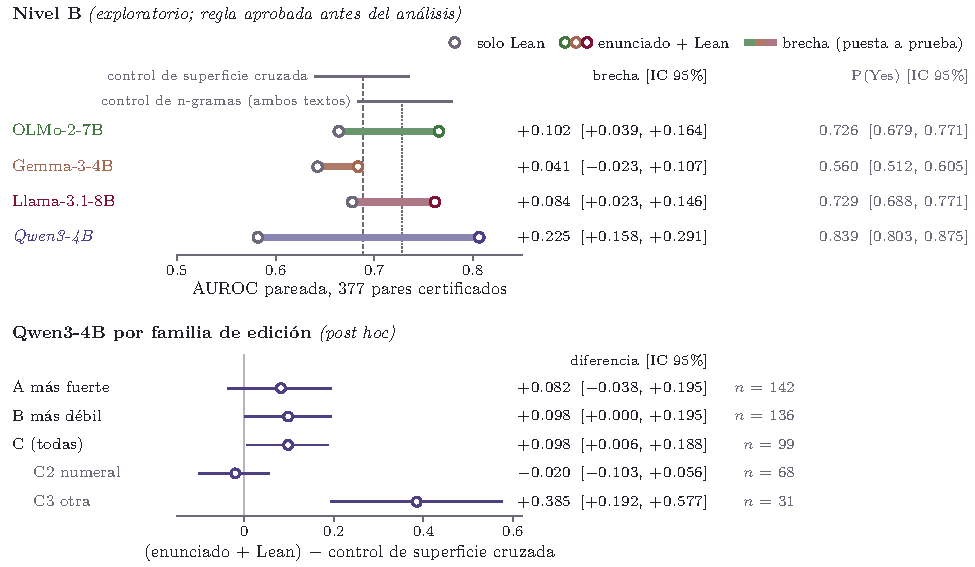
\includegraphics[width=\linewidth]{figuras_v3/nivel_b_es.pdf}
\caption{Nivel B. Arriba: AUROC pareada de la sonda que lee el Lean solo (gris) y el enunciado con el Lean (color del modelo); la barra entre ambos es la brecha puesta a prueba, con su intervalo en la primera columna y el P(Yes) del propio modelo en la segunda. Las líneas discontinua y punteada son los controles de superficie cruzada y de n-gramas, con sus intervalos encima. Abajo: \vr{full} menos superficie cruzada en Qwen3-4B por familia de edición (post hoc).}
\label{fig:b}
\end{figure}

% ------------------------------------------------------------------ 6
\section{Nivel C: ProofNetVerif y transferencia}

\paragraph{Datos.}
ProofNetVerif \citep{proofnetverif} contiene 3752 pares de enunciado y formalización en Lean, 1142 de ellos etiquetados
como adecuados. Según nuestro conteo, los pares se reparten en 361 enunciados, 217 de los cuales tienen formalizaciones tanto adecuadas como inadecuadas.
Las particiones y el bootstrap se agrupan por enunciado, de modo que la muestra efectiva es de 361 grupos.

\begin{table}[h]
\centering
\caption{Nivel C. Qwen3-4B se corrió bajo la regla aprobada y es reportable bajo ella; Llama-3.1-8B se corrió
después y es exploratorio. Una prueba de permutación de comprobación de cada AUROC, con 20 permutaciones, devolvió su mínimo, $p = 0.048$, en
ambos modelos. El valor de transferencia de Llama-3.1-8B corresponde a la capa seleccionada, la 9 de 32; véase el texto.}
\label{tab:c}
\vspace{2pt}
\begin{tabular}{@{}lcc@{}}
\toprule
 & Qwen3-4B & Llama-3.1-8B\\
\midrule
\vr{full}                               & 0.832 [0.807, 0.855] & 0.791 [0.766, 0.819]\\
\vr{lean\_only}                         & 0.678 & 0.664\\
$\D$                                    & +0.154 [+0.121, +0.187] & +0.127 [+0.090, +0.165]\\
$\D$ dentro del mismo enunciado         & +0.177 [+0.141, +0.213] & +0.151 [+0.114, +0.195]\\
\vr{full} $-$ \vr{nl\_mismatched}       & +0.202 [+0.170, +0.234] & +0.175 [+0.138, +0.214]\\
\vr{full} $-$ P(Yes)                    & +0.044 [+0.020, +0.069] & +0.108 [+0.066, +0.150]\\
\vr{full} $-$ apilado                 & +0.146 [+0.115, +0.176] & +0.111 [+0.079, +0.145]\\
\vr{full} $-$ n-gramas de ambos textos       & +0.144 [+0.105, +0.185] & +0.103 [+0.063, +0.148]\\
\midrule
Transferencia desde CriticLeanBench, $\D_T$ & +0.222 [+0.176, +0.267] & −0.017 [−0.064, +0.030]\\
\bottomrule
\end{tabular}
\end{table}

\paragraph{Resultado.}
En ambos modelos la etiqueta es decodificable linealmente de las activaciones de \vr{full} mejor que del Lean solo.
La brecha persiste dentro del mismo enunciado, donde el enunciado no puede aportar ni dificultad ni fuente. En
Qwen3-4B sobrevive además a los n-gramas de superficie de ambos textos (+0.144 \ic{0.105}{0.185}) y al control
apilado (+0.146 \ic{0.115}{0.176}). Una segunda implementación, escrita sin acceso a la primera, da +0.15354
\ic{0.12102}{0.18714}.

\paragraph{Transferencia.}
Una sonda entrenada solo con CriticLeanBench y aplicada sin cambios a ProofNetVerif separa los pares en Qwen3-4B
(\vr{full} 0.761, \vr{lean\_only} 0.539). En Llama-3.1-8B, en la capa seleccionada en CriticLeanBench, no los separa.
Esa capa es la capa 9 de 32, el máximo de una curva de selección casi plana. Allí \vr{full} es 0.527 y
\vr{lean\_only}, en su propia capa seleccionada, es 0.544. En la misma corrida los valores de transferencia en capas
posteriores son más altos. Van de 0.60 a 0.67 para \vr{full} desde la capa 11 en adelante, frente a un máximo de
0.55 para \vr{lean\_only}. Esos valores son post hoc y sin intervalos, y no sacamos ninguna conclusión sobre la
transferencia en este modelo.

El Nivel~C no se restringe a formalizaciones que compilan. Entre sus negativos hay, por tanto, candidatos mal
tipados, lo que favorece a la sonda de solo Lean.

% ------------------------------------------------------------------ 7
\section{Lo que dicen los tres niveles en conjunto}

\begin{table}[h]
\centering
\caption{Estatus de la evidencia. «Pares modelo--lectura» cuenta los signos de las ocho estimaciones prerregistradas de la Tabla~\ref{tab:a}.}
\label{tab:conjunta}
\vspace{2pt}
\begin{tabularx}{\linewidth}{@{}lXXX@{}}
\toprule
 & A: CriticLeanBench & B: pares certificados & C: ProofNetVerif\\
\midrule
Etiquetas & validadas por humanos & del generador, certificadas por Lean & humanas, un solo anotador\\
Estatus & prerregistrado & exploratorio & regla aprobada de antemano (un modelo)\\
Signo de $\D$ & positivo en 7 de 8 pares modelo--lectura & positivo en 4 de 4 & positivo en 2 de 2\\
Resultado bajo su regla & no confirmado por modelo; media de los cuatro +0.045 [0.021, 0.069] con (ii) y +0.029 [−0.000, 0.058] con (i), post hoc & en el último token, 3 positivos con potencia reducida, 1 nulo & positivo\\
Amenaza principal & ruido de etiquetas y estilo & n-gramas de ambos textos, que solo Qwen3-4B supera; superficie en las ediciones de numeral; P(Yes) iguala a la sonda en Qwen3-4B & contaminación\\
\bottomrule
\end{tabularx}
\end{table}

El signo de la brecha es el mismo en casi todos los escenarios que examinamos. Leer el enunciado junto con el Lean
separa mejor que leer el Lean solo. Los niveles difieren, sin embargo, en cuánto autoriza cada uno. El Nivel~A es
la única prueba prerregistrada, y no pasó. El Nivel~B tiene el diseño más limpio, con el enunciado fijo y las
etiquetas certificadas por Lean, pero es un lote de desarrollo y parte de su efecto es de superficie. En el Nivel~C
el efecto es grande y, para Qwen3, la protección contra la memorización es la más débil. Ningún nivel sostiene por
sí solo la afirmación de que la adecuación es decodificable linealmente de modelos congelados más allá del Lean
solo.
Tomados en conjunto, justifican volver a hacer la pregunta con datos que los modelos no pueden haber visto.

% ------------------------------------------------------------------ 8
\begin{table}[h]
\centering
\caption{Controles por nivel. AUROC del control por sí solo, o \vr{full} menos el control donde lleva signo. «No corrido» significa que el control no existe para ese nivel.}
\label{tab:controlesnivel}
\vspace{2pt}
{\small
\begin{tabularx}{\linewidth}{@{}lXXX@{}}
\toprule
Control & A & B (último token) & C\\
\midrule
n-gramas & solo del Lean: 0.682, a la par de \vr{lean\_only} (0.678 a 0.688) & de ambos textos: 0.729 & \vr{full} menos: +0.144 Qwen3-4B, +0.103 Llama-3.1\\
Superficie cruzada & no corrido & 0.688 & no corrido\\
Apilado & Tabla~\ref{tab:a} & no aplica (\vr{nl\_only} es 0.500) & \vr{full} menos: +0.146, +0.111\\
\vr{nl\_mismatched} & no analizado & 0.506 a 0.537 & \vr{full} menos: +0.202, +0.175\\
P(Yes) & 0.47 a 0.51 en OLMo-2, Gemma-3 y Llama-3.1; 0.70 y 0.72 en Qwen3-4B y Qwen3-8B; no interpretable en DeepSeek-Prover-V2 & 0.839, 0.726, 0.729, 0.560 (orden de la Tabla~\ref{tab:b}) & 0.788 en Qwen3-4B\\
Pesos aleatorios & solo Qwen3-4B & no corrido & no corrido\\
bge-m3 & corrido & no corrido & no corrido\\
\bottomrule
\end{tabularx}}
\end{table}

\section{Limitaciones}

\paragraph{Contaminación.}
Parte de los datos era pública antes del lanzamiento de algunos de los modelos. ProofNetVerif se describió en junio
de 2024 y está en Hugging Face desde febrero de 2025, es decir, antes del lanzamiento de Qwen3 y alrededor o
después del lanzamiento de Llama-3.1. En el Nivel~B, formal-conjectures se hizo público en mayo de 2025. Según
nuestra datación, y con una excepción conocida, los enunciados en Lean del lote no eran públicos antes del
lanzamiento de los cuatro modelos sondeados allí. La excepción es un origen cuyo enunciado casi idéntico está en
Mathlib desde julio de 2024. No se revisaron versiones anteriores de los enunciados de FormalMATH-Lite. Los
enunciados en lenguaje natural, en cambio, son más antiguos en unos 210 de los 256 orígenes, donde los problemas
eran conocidos y sus formalizaciones no.

\paragraph{Etiquetas.}
Las etiquetas tienen una debilidad distinta en cada nivel. El Nivel~A usa las etiquetas del benchmark, propuestas
por un modelo y validadas por revisores humanos, y algunas de ellas descansan en criterios amplios. Las etiquetas
del Nivel~B provienen del generador y están certificadas por Lean. El cribado que retiró los originales no
adecuados, sin embargo, lo hizo un modelo, y una de las fuentes del lote, FormalMATH-Lite, tiene defectos
documentados \citep{ammanamanchi2026faults}.
El Nivel~C tiene un único anotador.

\begin{pendiente}
Está en curso una revisión humana a ciegas de 80 ítems (40 del Nivel~B, 40 del Nivel~C), con umbrales de acuerdo fijados de antemano.
Sus tasas de acuerdo se reportarán aquí y acotarán el ruido de etiquetas de ambos niveles.
\end{pendiente}

\paragraph{Potencia.}
Las muestras son de 450 filas por modelo en el Nivel~A, 256 orígenes en el Nivel~B y 361 grupos en el Nivel~C.

\paragraph{Método.}
Las sondas son lineales y la evidencia es correlacional. En Qwen3-4B, en el Nivel~B, la propia respuesta del modelo
separa tan bien como la sonda. No hemos intervenido sobre ninguna dirección.

\paragraph{Decisiones a posteriori.}
Varios análisis se decidieron después de ver resultados. Son la división de la familia C, la exclusión de C2, las
corridas en Qwen3-8B y en Llama en el Nivel~C, los tres modelos posteriores y la segunda lectura del Nivel~B, el
control por fuente, el bootstrap conjunto, las figuras capa por capa, y los mapas con sus estadísticos de región y
su nulo de intercambio. Están rotulados como tales donde aparecen.

% ------------------------------------------------------------------ 9
\section{Conclusión}

Nuestra pregunta era si las activaciones de un modelo congelado separan una formalización que dice lo que se quiso
decir de otra que no lo dice, más allá de lo que revela el texto formal por sí solo. La respuesta que el piloto
sostiene es estrecha. La brecha es positiva en la mayoría de los escenarios que probamos, de unos pocos puntos de
AUROC en el Nivel~A, y está ausente con pesos aleatorios o con embeddings genéricos. Varios de sus intervalos, sin
embargo, incluyen el cero. Son la mayoría de los de la lectura en el último token en el Nivel~A, donde Llama-3.1 es
negativo, y el de Gemma-3 en el último token en el Nivel~B. La transferencia en Llama-3.1, en la capa
seleccionada, es indistinguible de cero. La brecha no pasó la prueba por modelo a la que nos comprometimos de
antemano. En los pares certificados, parte de ella es un numeral que falta en el enunciado, y en el Nivel~C los
datos eran públicos antes del lanzamiento de uno de los dos modelos.

El piloto arroja así una señal pequeña y una lista de las maneras en que podría ser un artefacto. El borrador de
protocolo del Apéndice~\ref{app:protocolo} está diseñado para eliminar o medir los elementos de superficie,
contaminación y etiquetas de esa lista. Todavía no se ocupa de un P(Yes) que iguala a la sonda. Los mapas de la
Figura~\ref{fig:escaner} muestran dónde la dirección de capa fija separa las clases. Si el modelo usa esa dirección
es una pregunta causal, que el sondeo no puede responder y que una intervención a lo largo de la dirección de la
sonda sí podría.

\paragraph{Uso de herramientas de IA.}
El código de análisis y la primera implementación de cada nivel se escribieron con asistentes de programación de IA,
bajo reglas fijadas por el primer autor. Él aprobó cada regla de decisión antes de que corriera su análisis, y los
resultados se compararán con una implementación que él escriba a mano antes de reportarse como hallazgos. Esa
comparación está pendiente. Los autores son responsables de todas las afirmaciones.

\paragraph{Código y datos.}
El repositorio se publicará con el preprint en \url{https://github.com/cmorregof}. Contendrá las reglas de decisión
con sus hashes y horas, los pares certificados, los rasgos de superficie cruzada y todos los archivos de resultados
citados aquí.


\bibliography{refs}
\bibliographystyle{tmlr}

\appendix
\section{Modelos y revisiones}\label{app:modelos}
\begin{table}[h]
\centering
\caption{Modelos, revisiones fijadas y número de posiciones del flujo residual leídas (embeddings más cada bloque).}
\vspace{2pt}
\begin{tabular}{@{}llcc@{}}
\toprule
Modelo & Identificador en Hugging Face & Revisión & Capas + emb.\\
\midrule
Qwen3-4B              & \vr{Qwen/Qwen3-4B}                         & \vr{1cfa9a72} & 37\\
Qwen3-8B              & \vr{Qwen/Qwen3-8B}                         & \vr{b968826d} & 37\\
OLMo-2-7B             & \vr{allenai/OLMo-2-1124-7B-Instruct}       & \vr{470b1fba} & 33\\
Gemma-3-4B            & \vr{google/gemma-3-4b-it}                  & \vr{093f9f38} & 35\\
Llama-3.1-8B          & \vr{meta-llama/Llama-3.1-8B-Instruct}      & \vr{0e9e39f2} & 33\\
DeepSeek-Prover-V2-7B & \vr{deepseek-ai/DeepSeek-Prover-V2-7B}     & \vr{a8d9e144} & 31\\
Goedel-Prover-V2-8B   & \vr{Goedel-LM/Goedel-Prover-V2-8B}         & \vr{dfd02e62} & 37\\
Kimina-7B             & \vr{AI-MO/Kimina-Autoformalizer-7B}        & \vr{ddd47cb4} & 29\\
\bottomrule
\end{tabular}
\end{table}

\section{Desviaciones y decisiones tardías}\label{app:desviaciones}

La lista que sigue sale de los informes de cada nivel. La bitácora del proyecto guarda una lista numerada más larga,
que se publicará con el repositorio, y nada de lo que hay aquí la reemplaza.

\begin{description}[leftmargin=1.2em]
\item[4 nov] En un solo día se escribieron tres versiones de la regla del Nivel~A. La tercera, firmada a las 22:29,
es la que se aplica aquí. Goedel-Prover-V2 y Kimina se habían corrido con la primera y se reportan como un primer
intento fallido.
\item[5 nov, 08:37] Se corrigió un error en la matriz de permutaciones de la lectura~(i) del script de análisis y
se volvió a correr DeepSeek-Prover-V2. La lectura~(ii) no se vio afectada.
\item[5 nov] Cuando los \emph{offsets} del tokenizador no cuadran con el texto, la extracción localiza los tokens
de Lean por prefijo. Esto cambió un solo modelo, DeepSeek-Prover-V2, en 1972 de sus 2000 prompts.
\item[5 nov] El primer autor confirmó dos cláusulas del documento del Nivel~A cuando ya se habían visto los
resultados de la lectura~(ii). Una es que un modelo puede pasar con cualquiera de las dos lecturas, y la otra, que
el metaanálisis se lee lectura por lectura. Las demás cláusulas de implementación de ese documento las redactó el
asistente de código.
\item[5 nov] Por razones de tiempo, las permutaciones usan un solver de Newton exacto en la base de la
descomposición en valores singulares, en lugar del solver de la biblioteca. El estadístico observado se calcula con
el mismo solver.
\item[5--6 nov] Un reinicio de la máquina hizo perder las permutaciones de la lectura~(i) de Gemma-3. El 6 de
noviembre el primer autor decidió no correrlas para Gemma-3 ni para Llama-3.1, porque la condición~(b) ya había
fallado allí. La extracción de Llama-3.1 se reanudó desde lo guardado tras un atasco de memoria.
\item[6 nov] En el Nivel~B una comprobación de superficie fijada de antemano no pasó (0.706 en los pares
certificados), y el lote se declaró exploratorio. Se corrigió un error de código en el control que puntúa el
original frente a su edición adecuada (0.520). La división de la familia C por tipo de edición se añadió ese mismo
día, después de los resultados.
\item[7--8 nov] Llama-3.1 en el Nivel~C, Qwen3-8B en el Nivel~A y tres modelos más en el Nivel~B se corrieron
después de los primeros resultados de cada nivel.
\item[9 nov] Se añadieron el control por fuente, el bootstrap conjunto, los mapas por capa y posición, sus
estadísticos de región y el nulo de intercambio. La hipótesis del borrador de protocolo pasó a exigir los dos
controles de superficie.
\end{description}

\section{Borrador de un protocolo confirmatorio sobre enunciados escritos después del piloto}\label{app:protocolo}

El piloto fija cuatro requisitos de una prueba limpia, y el protocolo que sigue está escrito para cumplirlos. El
enunciado se mantiene constante y las etiquetas están certificadas por Lean. La comparación se hace con los dos
controles de superficie, rasgos de superficie cruzada y n-gramas simples, además de con el Lean. Los enunciados son
tales que los modelos no pueden haberlos visto.

\begin{description}[leftmargin=1.2em]
\item[Hipótesis] En Qwen3-4B, en el último token y con la capa elegida por validación cruzada anidada, la AUROC
pareada de \vr{full} supera a ambos controles de superficie. Es decir, \vr{full} menos superficie cruzada $> 0$ y
\vr{full} menos n-gramas simples de los dos textos $> 0$, con cada intervalo por completo por encima de cero.
\item[Población] Pares de las familias A, B y C3. Las ediciones de numeral se reportan por separado.
\item[Datos] Enunciados añadidos a formal-conjectures después del 23 de octubre de 2026 (commit \vr{c094b979}, la copia usada en el piloto),
procesados con el generador y el certificador del piloto, congelados por hash. Por construcción ninguno estuvo en el
piloto, y todos son posteriores al lanzamiento de cada modelo sondeado aquí.
\item[Instantánea] 1 de noviembre de 2027, 00:00 UTC, prorrogada una sola vez hasta el 1 de febrero de 2028 si hay menos de 200 orígenes
disponibles. Con unos 300 orígenes el efecto mínimo detectable es de alrededor de 0.08 ($\alpha = 0.025$
unilateral, potencia 0.8). Esa cifra se calculó para el contraste con la superficie cruzada sola y tiene que
recalcularse para la hipótesis de dos controles.
\item[Réplica] El mismo contraste combinado sobre los cuatro modelos prerregistrados del Nivel~A.
\item[Verificaciones] 100 permutaciones dentro de cada par, una implementación independiente escrita a mano que debe
coincidir dentro de 0.005 y llegar a la misma decisión, y una revisión humana a ciegas de las etiquetas.
\end{description}

\begin{pendiente}
El protocolo es un borrador. Se firma, y su SHA-256 se registra, solo después de que concluyan la revisión a ciegas y
la comparación con la implementación escrita a mano.
\end{pendiente}

% ------------------------------------------------------------------ 10

\end{document}
